\chapter{Descente de gradient}
\label{ch:descente}

\begin{lecture}
Le coût dépend des trois coefficients. Encore faut-il déterminer dans quel sens les déplacer. La quantité qui l'indique prend ici une forme simple : l'erreur commise
sur un élève, multipliée par sa note. Les valeurs citées proviennent d'une
descente exécutée sur les mille six cents élèves.
\end{lecture}

\section{Correction à appliquer}

Le coût $J(w)$ atteint son minimum quelque part dans l'espace des coefficients,
et la descente doit s'y rendre sans en connaître la position. Ce qu'elle peut
mesurer, en revanche, c'est la pente du coût au point où elle se trouve : de
combien $J$ varie lorsqu'on modifie légèrement un coefficient.

Cette pente est la \emph{dérivée partielle} $\partial J/\partial w_j$, variation
de $J$ par unité de $w_j$, les autres coefficients restant fixés. Son signe suffit
à décider du sens. Positive, elle indique qu'augmenter $w_j$ augmente le coût, et
qu'il faut donc le diminuer ; négative, elle indique l'inverse. Se déplacer à
l'opposé de la pente fait baisser $J$, pourvu que le déplacement reste assez
petit pour que la pente mesurée décrive encore le terrain.

\[
  \ann{accent}{w_j}{\annl{nouvelle}\\ \annl{valeur}}
  \;\longleftarrow\;
  \ann{accent}{w_j}{\annl{ancienne}\\ \annl{valeur}}
  \;-\;
  \ann{warning}{\alpha}{\annl{taux}\\ \annl{d'apprentissage}}
  \ann{rulecolor}{\frac{\partial J}{\partial w_j}}{\annl{pente du coût}\\ \annl{en ce point}}
  \qquad\text{pour tous les } j \text{ à la fois.}
\]
Tout l'algorithme tient dans ce signe moins. Le facteur $\alpha$ fixe la longueur
du pas : c'est le \emph{taux d'apprentissage}, seul paramètre que l'utilisateur
règle lui-même.

Les coefficients sont corrigés simultanément, à partir des mêmes valeurs
antérieures. Corriger $w_0$ puis calculer la correction de $w_1$ avec le $w_0$
déjà modifié évaluerait les deux dérivées en deux points distincts.

Reste à calculer cette pente. Pour le coût logistique, elle prend une forme dont
tous les termes s'interprètent, et que le chapitre~\ref{ch:gradient} établit :
\[
  \frac{\partial J}{\partial w_j}
  =\ann{rulecolor}{\frac{1}{m}\sum_{i=1}^{m}}{\annl{moyenne sur}\\ \annl{les $m$ élèves}}
   \;\ann{warning}{\bigl(p_i-y_i\bigr)}{\annl{erreur sur l'élève $i$}\\ \annl{annoncé moins observé}}
   \;\ann{accent}{x_{ij}}{\annl{sa note dans}\\ \annl{la matière $j$}}
\]

$p_i-y_i$ est l'erreur commise sur l'élève $i$ : la probabilité annoncée moins la
réponse observée. Elle vaut $-0{,}9$ pour un \Gryf auquel le modèle
n'accorde que $0{,}1$, et $-0{,}01$ pour un \Gryf déjà reconnu à $0{,}99$.
La correction se trouve négligeable pour un élève correctement classé, maximale
pour un élève classé dans l'autre catégorie avec une probabilité élevée.

$x_{ij}$ est sa note dans la matière $j$. Elle pondère la contribution de
l'erreur au coefficient $j$ : un élève aux notes extrêmes contribue fortement, un
élève moyen, dont la note standardisée avoisine zéro, presque pas.

\section{Premier pas de la descente}

La descente part ici de coefficients nuls. Quel que soit ce départ, le point d'arrivée reste le même, la surface du coût
ayant un fond unique (ch.~\ref{ch:convexite}) ; partir de zéro rend en outre le
premier tour calculable à la main, tous les scores valant alors zéro et toutes
les probabilités $0{,}5$. La correction du biais s'écrit alors,
puisque $x_{i0}$ vaut $1$ pour tout le monde,
\[
  \frac{\partial J}{\partial w_0}
  =\frac{1}{m}\sum_{i=1}^{m}
   \bigl(\ann{warning}{0{,}5}{\annl{annoncé}}-\ann{accent}{y_i}{\annl{observé}}\bigr)
  =\ann{warning}{0{,}5}{\annl{proportion}\\ \annl{annoncée}}
   -\ann{accent}{\frac{327}{1\,600}}{\annl{proportion}\\ \annl{réelle}}
  =0{,}5-0{,}2044
  =0{,}2956
\]
\begin{releve}
La descente donne exactement cette valeur, $327$ élèves sur $1\,600$ étant
\Gryf. Avec $\alpha=1$, le biais passe de $0$ à $-0{,}2956$.
\end{releve}

Le modèle annonçait $50\,\%$ de \Gryf pour une fréquence observée de
$20{,}44\,\%$. Le biais diminue, et continuera de diminuer tant que la
moyenne annoncée dépassera cette fréquence.

\begin{table}[htbp]
\centering
\begin{tabular}{rrrrr}
\toprule
itération & $w_0$ (biais) & $w_1$ (\Herb) & $w_2$ (\Runes) & coût $J$ \\
\midrule
$0$   & $0{,}0000$  & $0{,}0000$  & $0{,}0000$ & $0{,}693147$ \\
$1$   & $-0{,}2956$ & $-0{,}2289$ & $0{,}1924$ & $0{,}538507$ \\
$2$   & $-0{,}5194$ & $-0{,}4005$ & $0{,}3364$ & $0{,}449297$ \\
$5$   & $-0{,}9622$ & $-0{,}7378$ & $0{,}6266$ & $0{,}325975$ \\
$10$  & $-1{,}3952$ & $-1{,}0678$ & $0{,}9338$ & $0{,}250029$ \\
$50$  & $-2{,}7318$ & $-2{,}0538$ & $1{,}9613$ & $0{,}143846$ \\
$400$ & $-4{,}7454$ & $-3{,}4535$ & $3{,}4688$ & $0{,}108113$ \\
\bottomrule
\end{tabular}
\caption{Descente réelle, $\alpha=1$, sur les $1\,600$ élèves. Le coût initial
vaut $\log 2$ (ch.~\ref{ch:cout}). Les signes des
coefficients se fixent dès le premier tour et ne changent plus : négatif pour
\Herb, positif pour \Runes.}
\label{tab:trace}
\end{table}

\section{Coût au fil des itérations}

Répéter l'opération précédente quatre cents fois produit une suite de coûts, dont
le tracé résume la descente entière. La baisse y est d'abord rapide, puis de plus
en plus lente, et cette forme se déduit de la formule de correction.

Au départ, chaque élève contribue autant que les autres : le modèle accorde
$0{,}5$ à tout le monde et se trompe ainsi de moitié sur chacun, si bien que les
mille six cents erreurs $p_i-y_i$ s'additionnent. À mesure que les probabilités s'ajustent,
l'erreur s'éteint pour les élèves que le modèle a placés du bon côté, et la
correction ne provient plus que des cas litigieux, qui sont peu nombreux. La somme qui commande le déplacement se vide ainsi de ses termes, tour après tour.

\begin{figure}[htbp]
\centering
\begin{tikzpicture}
\begin{axis}[courseplot,height=6.4cm,axis lines=left,
  xlabel={itération},ylabel={coût $J$},xmin=0,xmax=400,ymin=0,ymax=.75]
  \addplot[accent,very thick,no markers] table[x=iter,y=cost] {data/cout.dat};
  \addplot[only marks,mark=*,warning,mark size=2.2pt]
    coordinates {(0,0.693147) (10,0.250029) (50,0.143846) (400,0.108113)};
\end{axis}
\end{tikzpicture}
\caption{Le coût moyen à chaque tour. Les points marquent les itérations $0$,
$10$, $50$ et $400$, dont le tableau~\ref{tab:trace} donne les coefficients. Les
dix premières couvrent les deux tiers de la baisse totale ; les trois cent
cinquante dernières n'agissent plus que sur la quatrième décimale.}
\label{fig:cout}
\end{figure}

\begin{figure}[htbp]
\centering
\begin{tikzpicture}
\begin{axis}[courseplot,height=5.6cm,axis lines=left,ymode=log,
  xlabel={itération},ylabel={longueur du gradient},xmin=0,xmax=400]
  \addplot[warning,very thick,no markers] table[x=iter,y=norm] {data/gradient.dat};
\end{axis}
\end{tikzpicture}
\caption{La longueur du gradient, en échelle logarithmique. Elle décroît
régulièrement : la surface s'aplatit à l'approche du minimum. C'est cette
quantité, ou la variation du coût, qui sert de critère d'arrêt.}
\label{fig:norme}
\end{figure}
\FloatBarrier

La seconde figure mesure cet épuisement directement : la longueur du gradient,
c'est-à-dire la taille de la correction appliquée à chaque tour. Elle passe de $0{,}42$ à $0{,}0026$ sur les quatre cents
itérations, soit une division par cent soixante. De cette décroissance vient le critère d'arrêt : une correction devenue assez petite laisse les
coefficients là où ils sont.

\section{Déplacement de la frontière}

La frontière $w_0+w_1x_1+w_2x_2=0$ se trace sous sa forme résolue,
\[
  x_2=-\frac{w_0+w_1x_1}{w_2},
\]
qui donne son ordonnée pour chaque abscisse. Reportée à trois moments de la
descente, elle occupe presque la même position, et il faut agrandir le tracé pour
séparer les trois droites.

\begin{figure}[htbp]
\centering
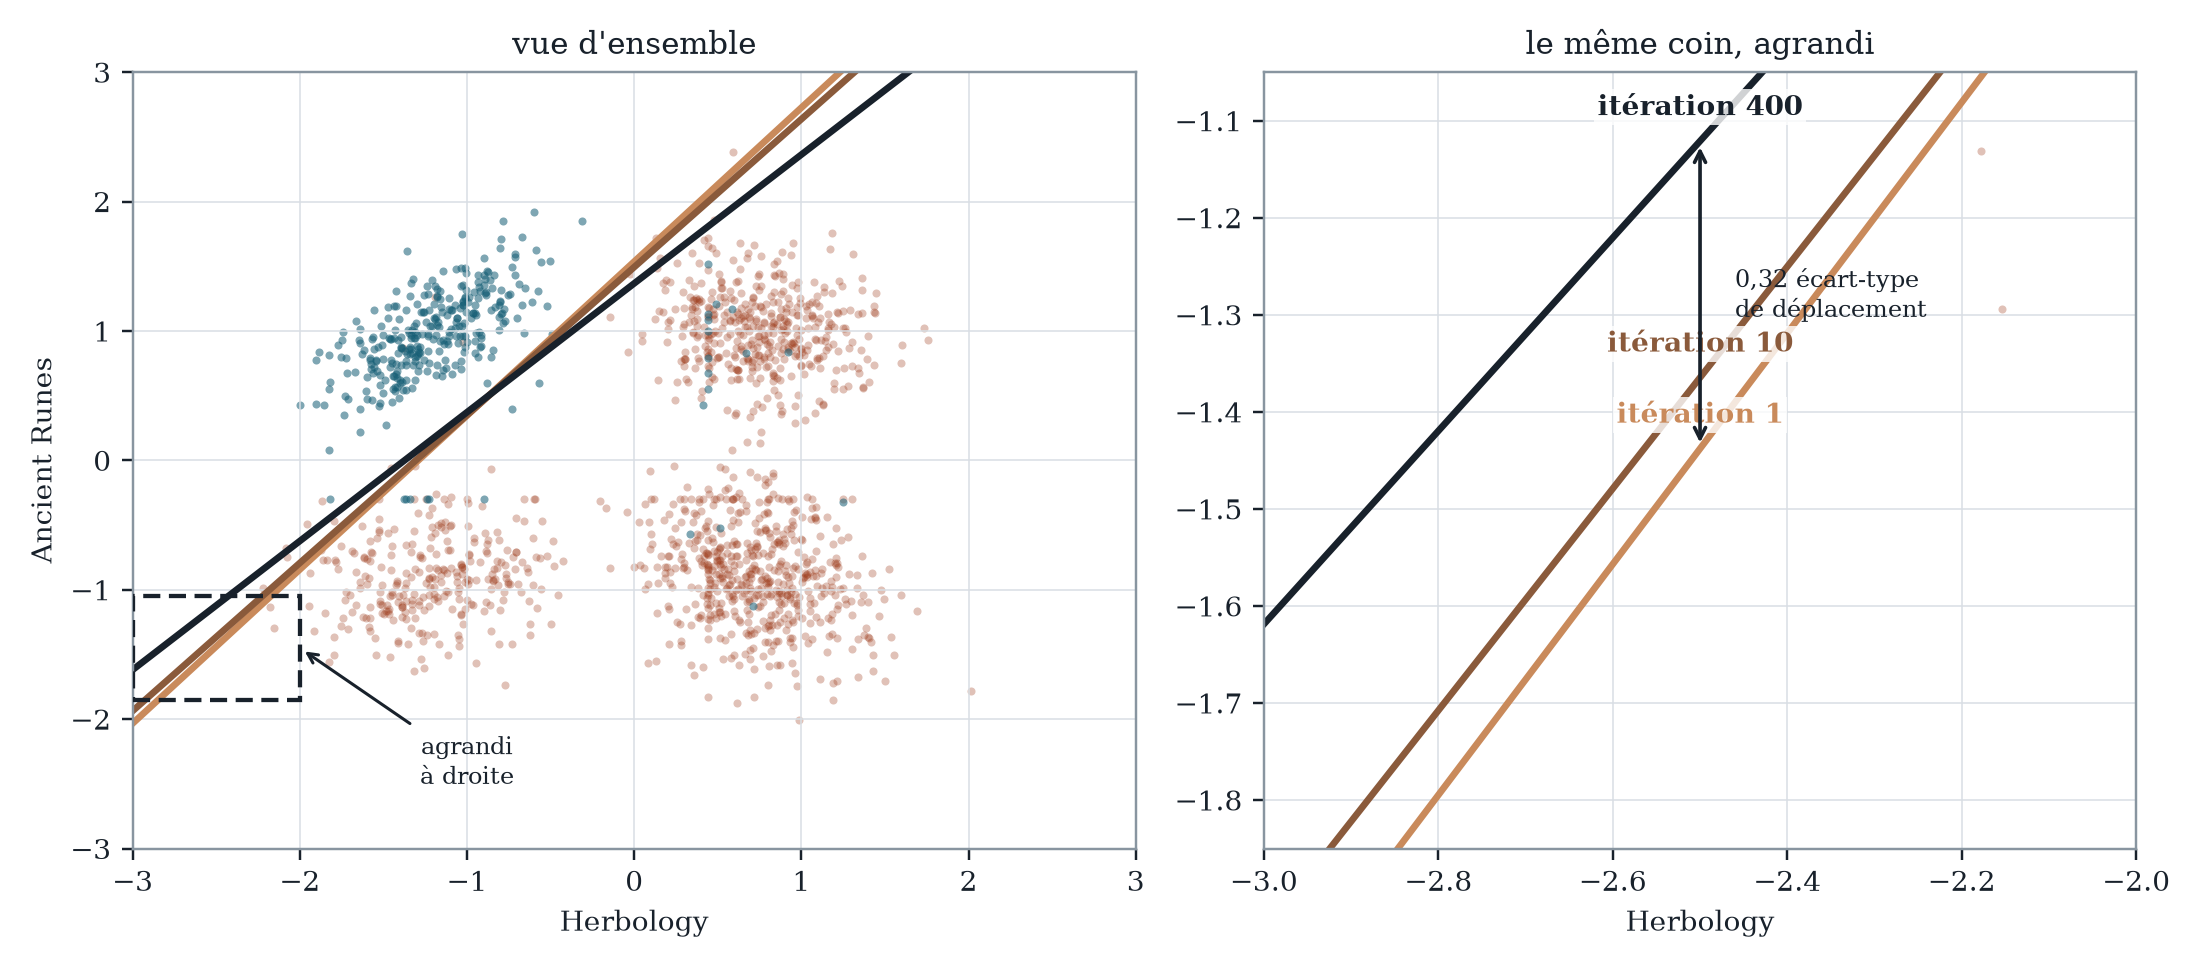
\includegraphics[width=\textwidth]{figures/zoom_droite.png}
\caption{La frontière aux itérations $1$, $10$ et $400$. À l'échelle du nuage,
les trois droites se confondent ; le rectangle agrandi les sépare. Elles pivotent
autour d'un point situé vers le centre du nuage, d'où un écart nul en ce point et
maximal sur les bords. Le déplacement total vaut un tiers d'écart-type.}
\label{fig:zoom}
\end{figure}
\FloatBarrier

Trois cent quatre-vingt-dix-neuf itérations pour un tiers d'écart-type : la
descente consacre donc l'essentiel de son travail à autre chose qu'au
déplacement de cette droite. Pour voir ce travail, il faut regarder la quantité
que la descente modifie réellement, la probabilité, qui est définie en tout point
du plan et pas seulement sur la frontière.

\section{Surface de probabilité}

À chaque point du plan des notes, le modèle associe une probabilité d'appartenir
à \Gryf. Porter cette probabilité en altitude au-dessus du point qui la produit
définit une surface, que les trois figures suivantes donnent aux itérations $1$,
$10$ et $400$.

Le premier tour montre une surface presque plane, traversant le nuage à
mi-hauteur : le modèle répond $0{,}5$ ou presque en tout point, sans distinguer
personne. Au dixième, deux plateaux se dégagent, l'un au-dessus du groupe des
\Gryf, l'autre au-dessus des trois autres, séparés par une pente encore large. Au
quatre centième, les plateaux sont établis et la transition tient sur moins d'un
demi-écart-type.

Une chose reste pourtant fixe d'une figure à l'autre : la ligne noire tracée à
mi-hauteur, où la surface vaut exactement $0{,}5$. Sa projection au sol est la frontière du paragraphe précédent, et c'est de là que
vient sa quasi-immobilité pendant que la surface, elle, change du tout au tout.

\begin{figure}[p]
\centering
\makebox[\textwidth][c]{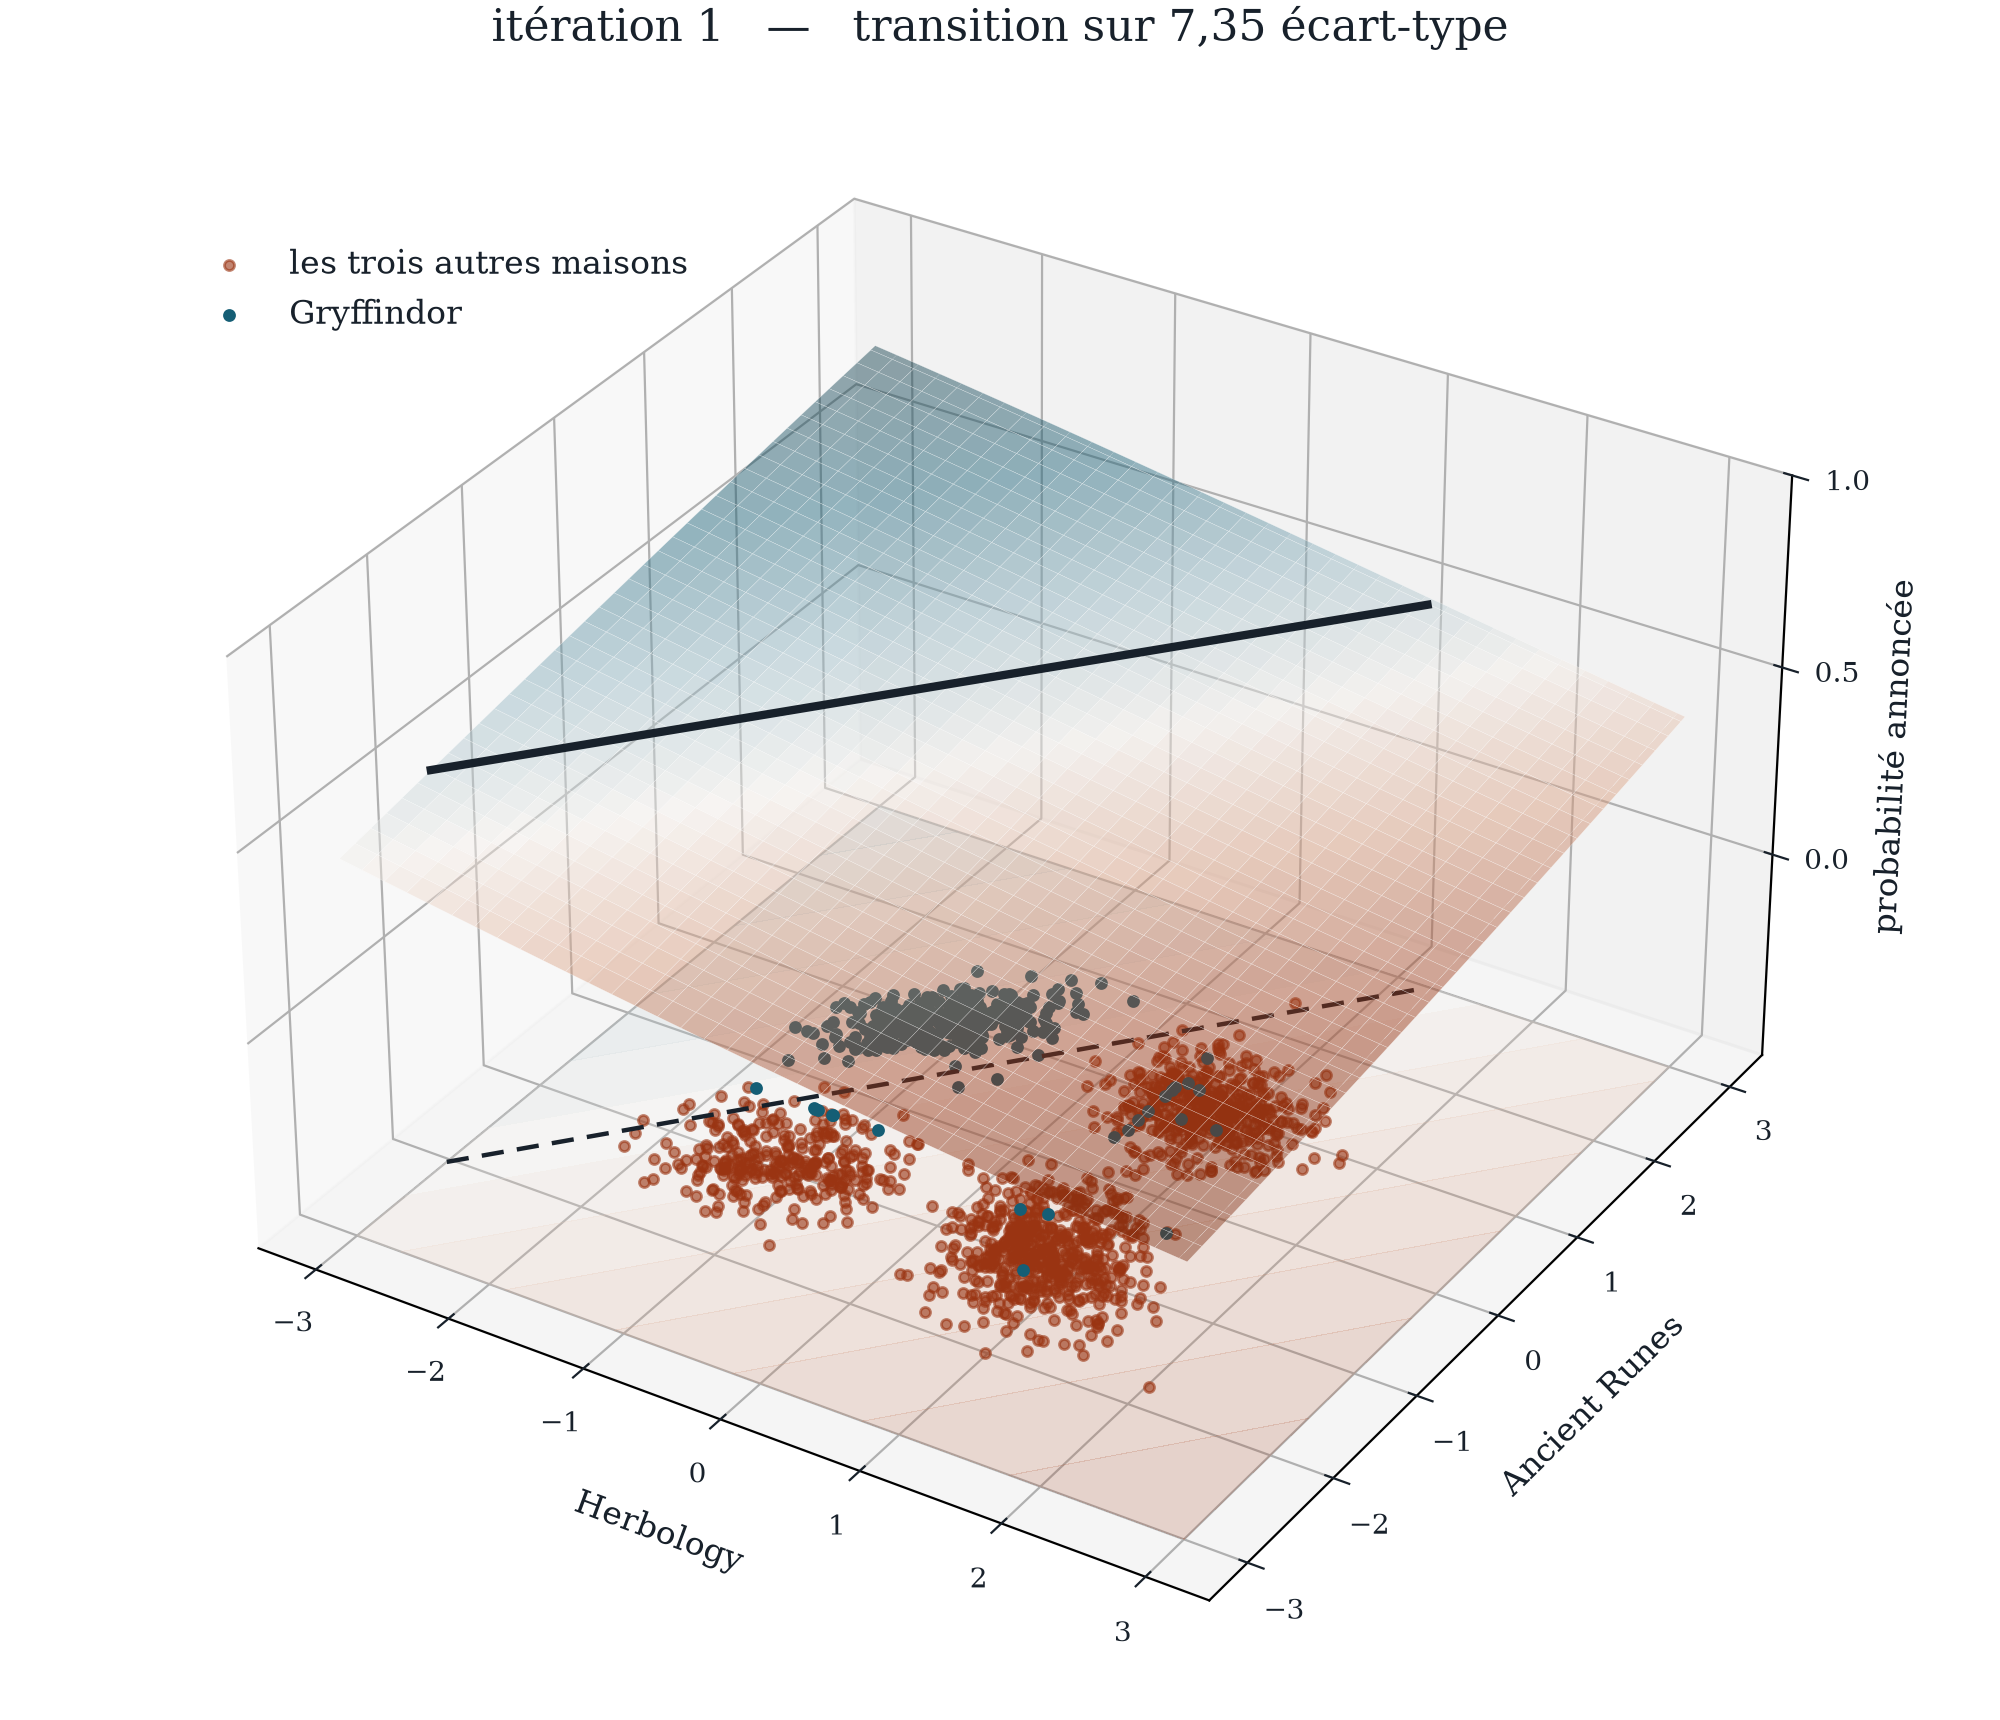
\includegraphics[width=1.28\textwidth]{figures/nappe_it1.png}}
\caption{Premier tour. La surface est presque plane et traverse le nuage à
mi-hauteur : le modèle répond $0{,}5$ ou presque en tout point, et la couleur
reste pâle au-dessus des quatre groupes d'élèves. La ligne noire marque les
$50\,\%$, le pointillé sa projection dans le plan des notes.}
\label{fig:champ}
\end{figure}

\begin{figure}[p]
\centering
\makebox[\textwidth][c]{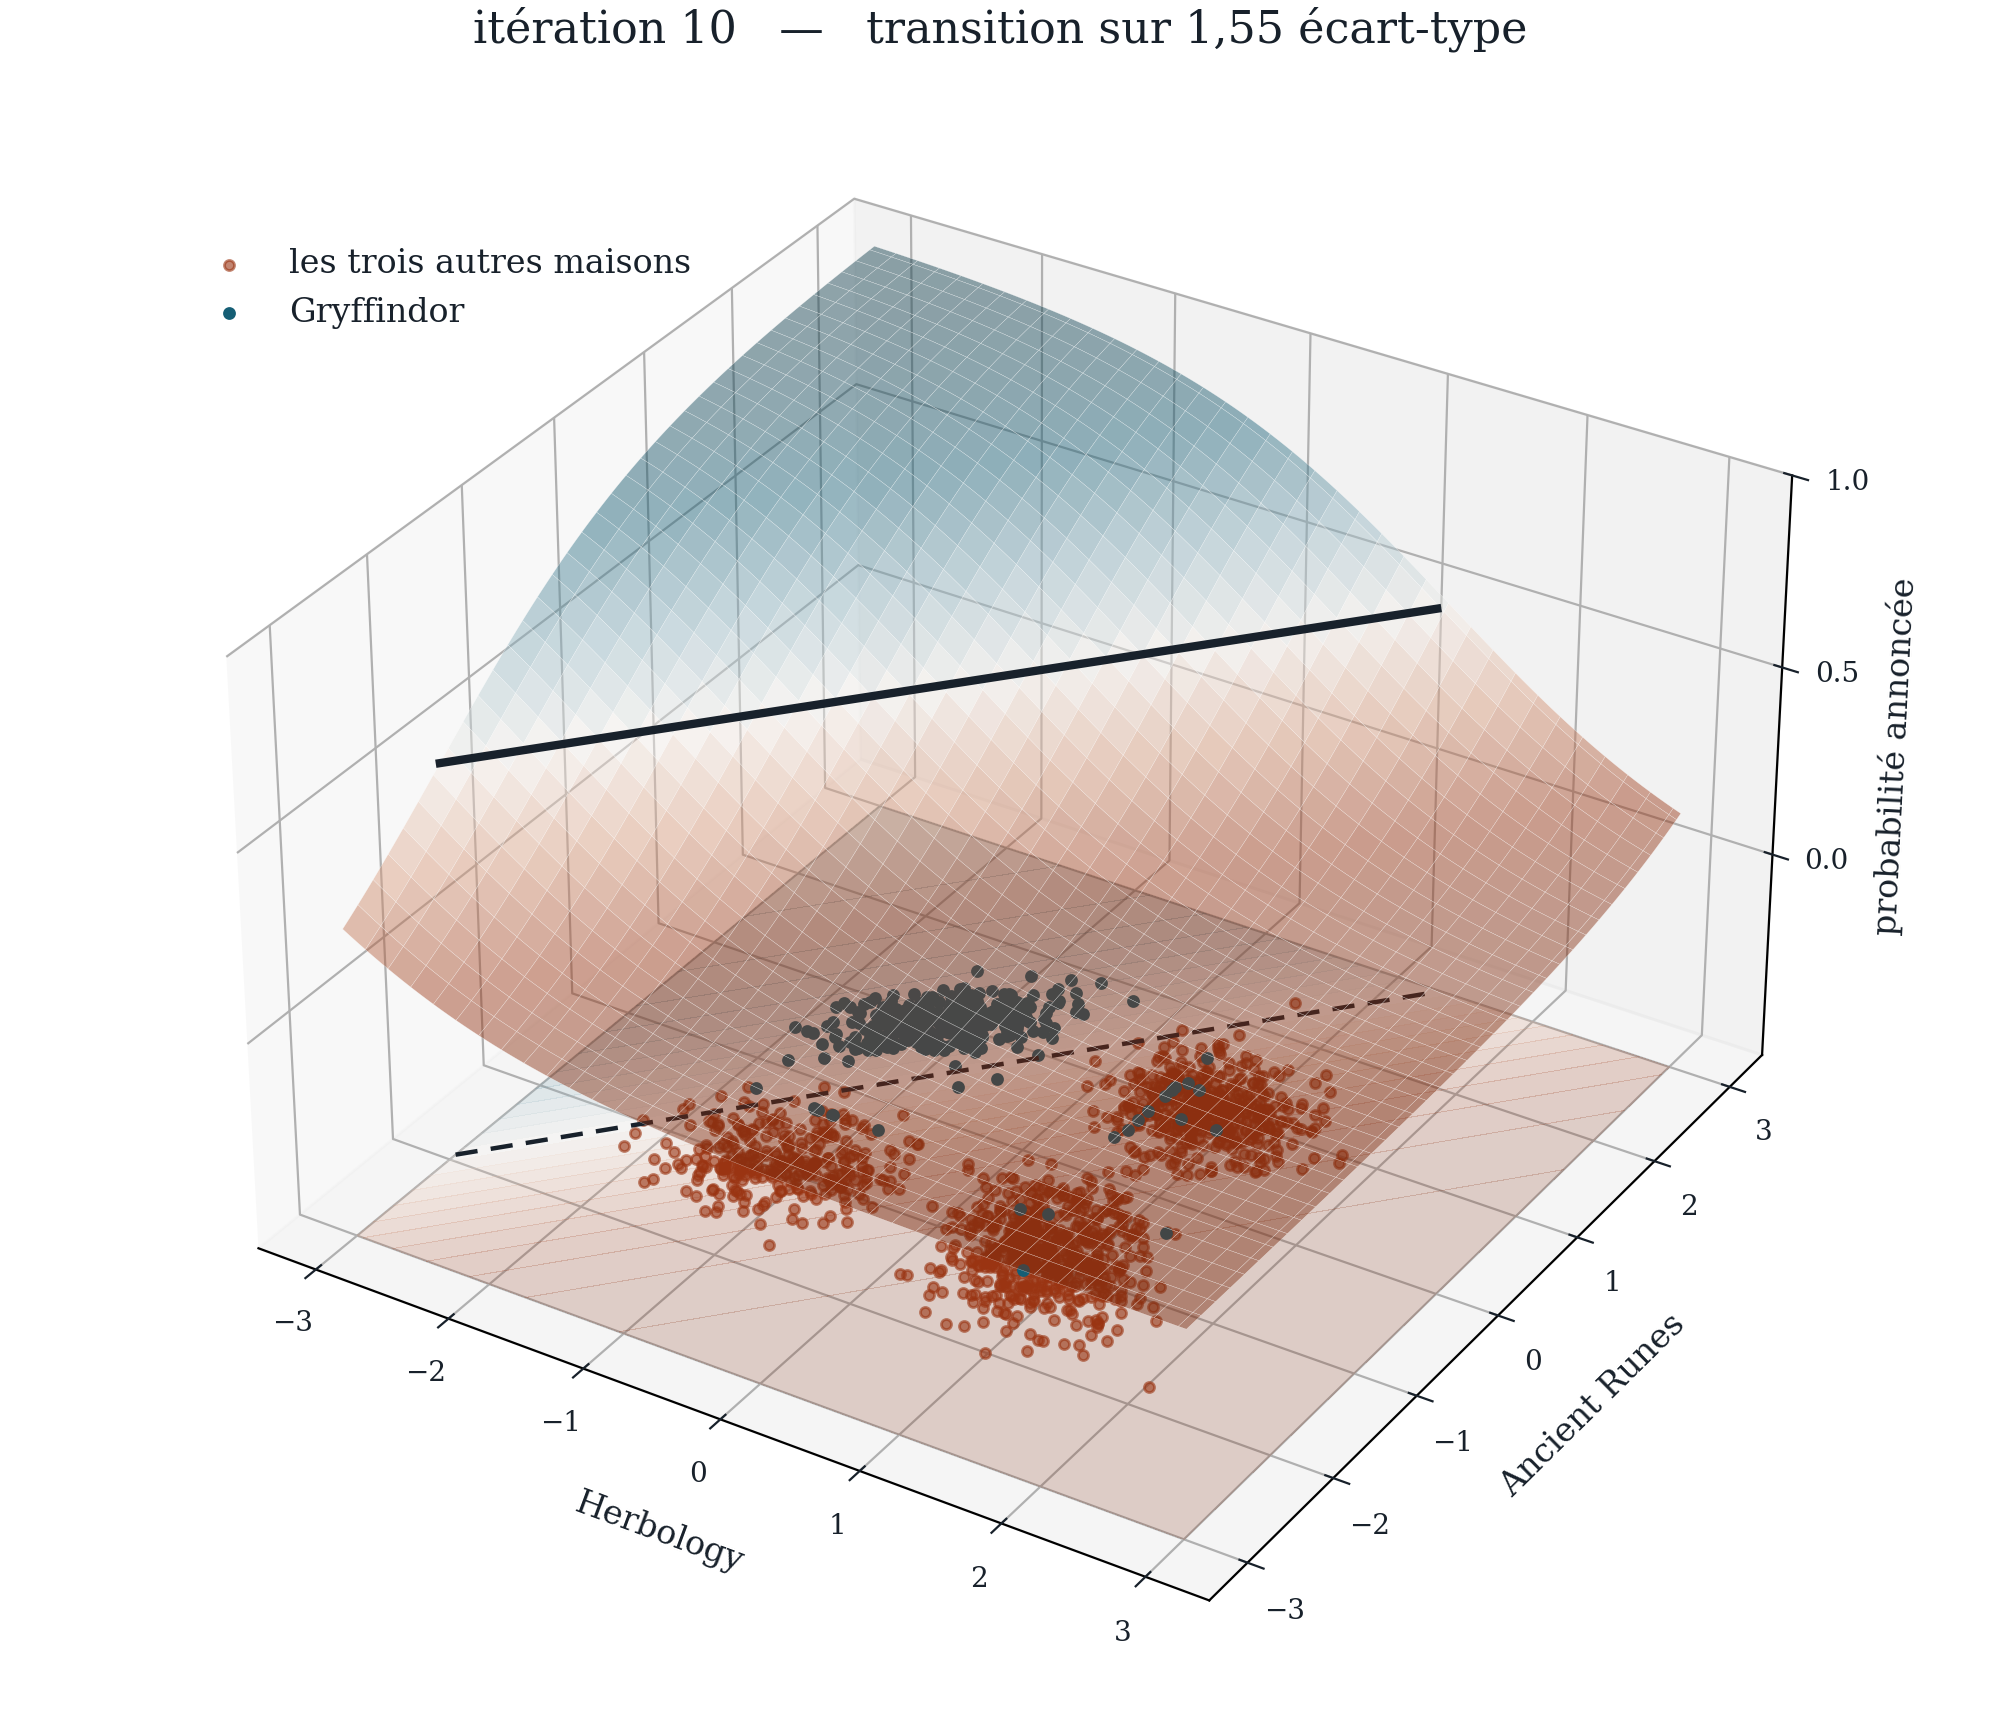
\includegraphics[width=1.28\textwidth]{figures/nappe_it10.png}}
\caption{Dixième tour. Les deux plateaux apparaissent, la transition s'est
resserrée d'un facteur cinq, et les couleurs se différencient au-dessus des
groupes.}
\label{fig:champ10}
\end{figure}

\begin{figure}[p]
\centering
\makebox[\textwidth][c]{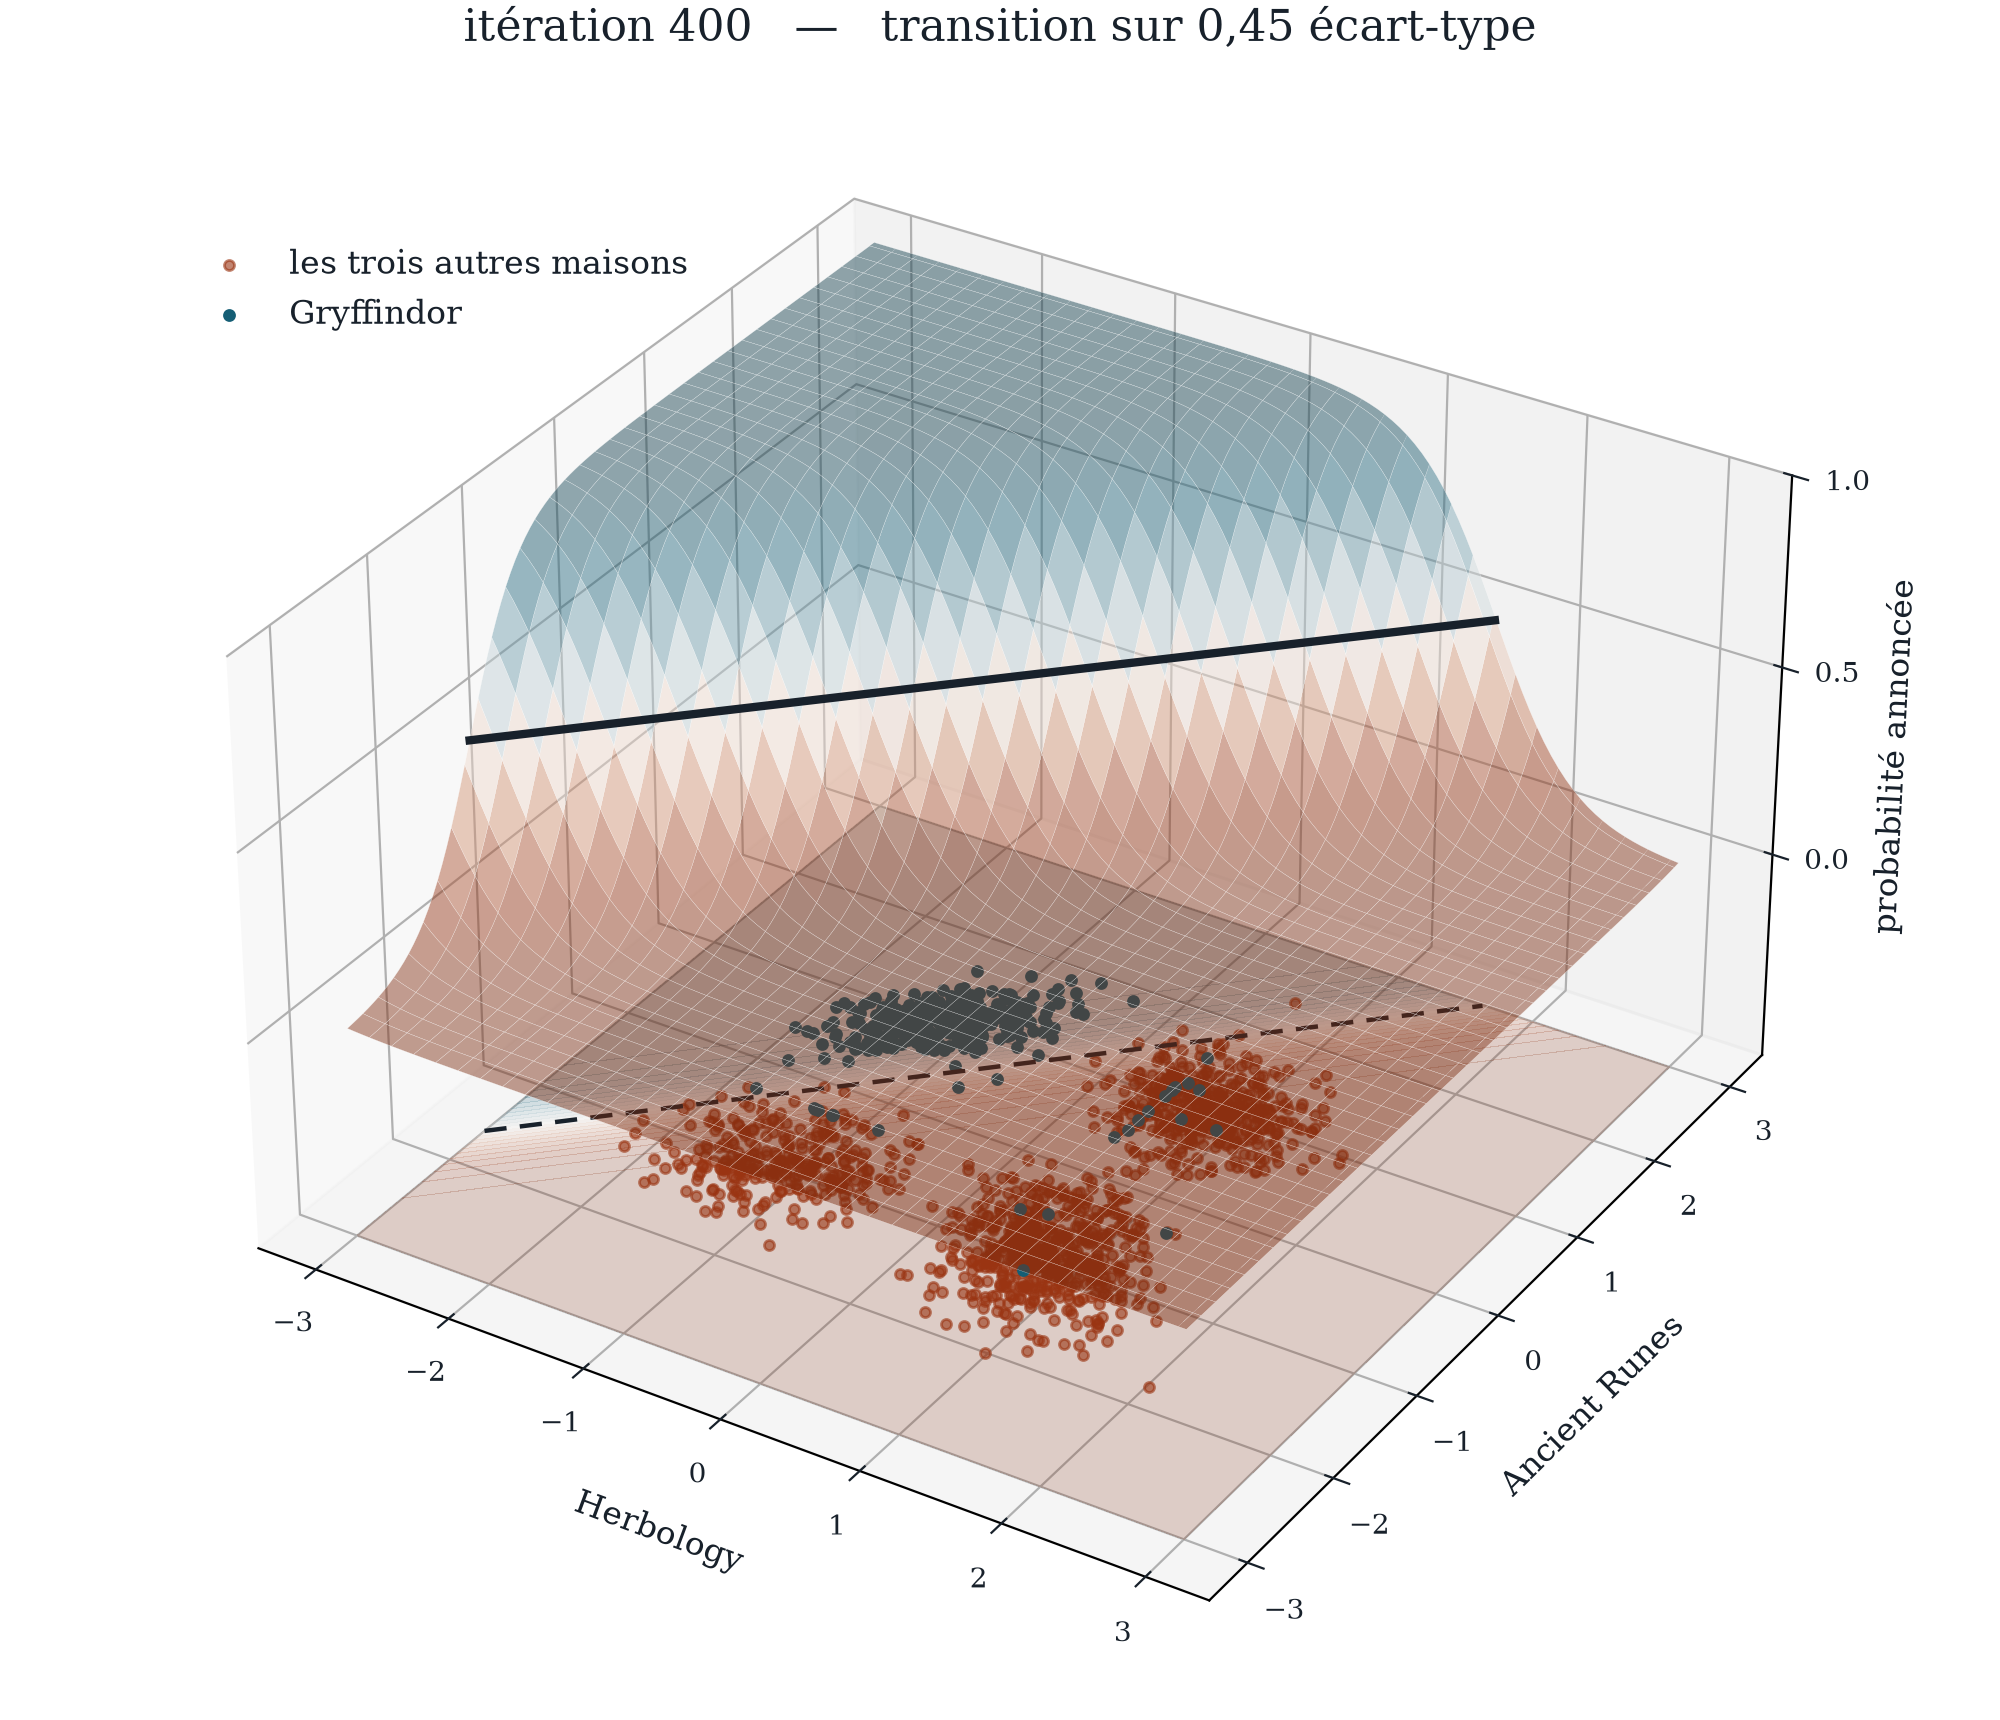
\includegraphics[width=1.28\textwidth]{figures/nappe_it400.png}}
\caption{Quatre centième tour. Le plateau bleu couvre le groupe des \Gryf,
le plateau brun les trois autres, et la transition tient sur moins d'un
demi-écart-type. La couleur indique la maison prédite ; les zones pâles sont
celles où la probabilité reste proche de $0{,}5$.}
\label{fig:champ400}
\end{figure}
\FloatBarrier

\section{Niveau \texorpdfstring{$0{,}5$}{0,5} de la sigmoïde}

Cette surface est la sigmoïde (ch.~\ref{ch:probabilite}) composée avec le
score. La frontière tracée jusqu'ici est le lieu où elle vaut exactement
$0{,}5$.

Notons $d$ la distance d'un élève à la frontière, comptée perpendiculairement et
affectée du signe du côté où il se situe. Alors
\[
  z=\|w\|\,d
  \qquad\text{donc}\qquad
  p=\sigma\bigl(\|w\|\,d\bigr) .
\]
Le rapport des coefficients fixe la position de la frontière (ch.~\ref{ch:nuage})
et leur norme $\|w\|$ fixe la rapidité avec laquelle la probabilité passe de $0$ à
$1$ de part et d'autre : les deux quantités agissent séparément. Relevée le long de cette
perpendiculaire,
la probabilité décrit toujours une sigmoïde, d'autant plus comprimée que
$\|w\|$ est grand.

\begin{figure}[htbp]
\centering
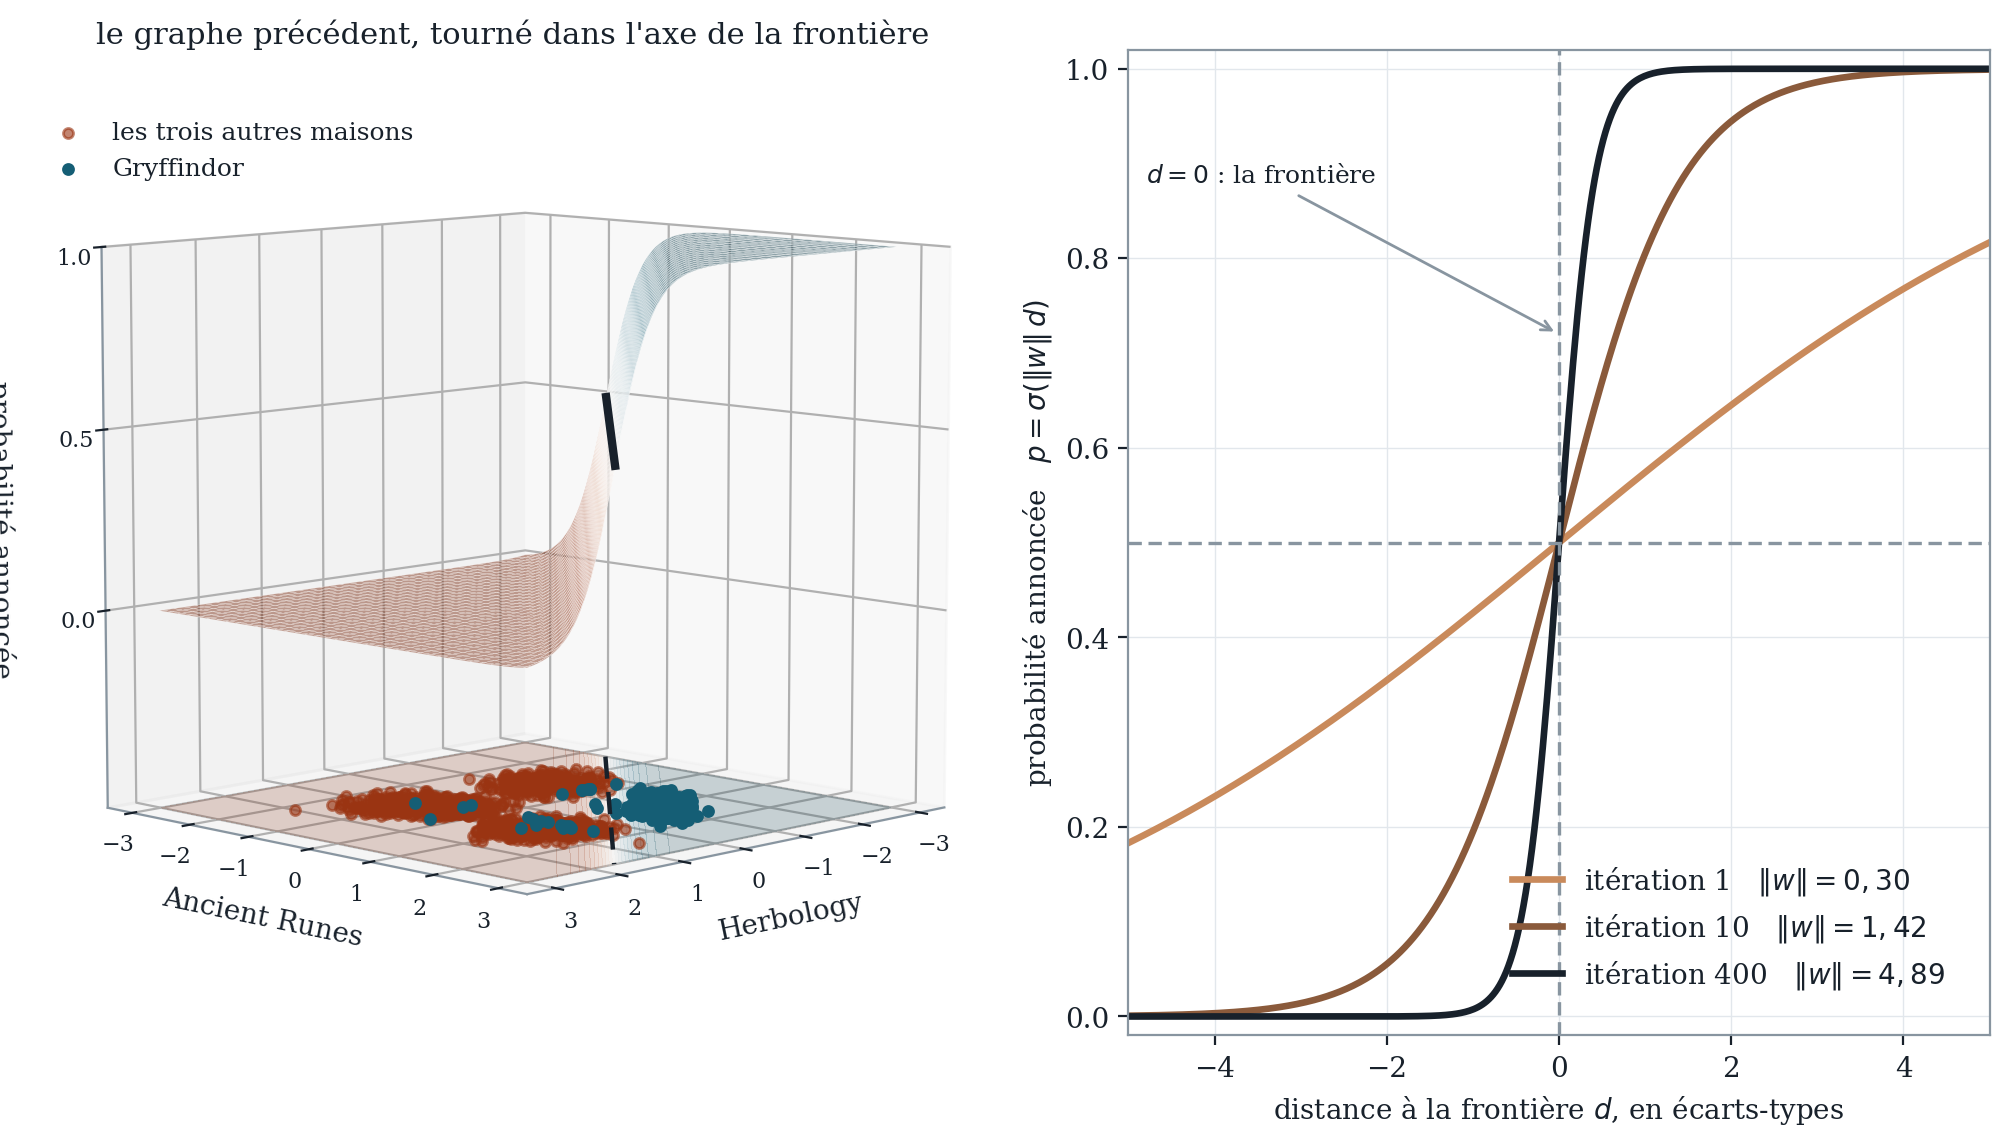
\includegraphics[width=\textwidth]{figures/coupe_sigmoide.png}
\caption{À gauche, le modèle vu de dessus et la direction perpendiculaire à la
frontière. À droite, la probabilité relevée le long de cette direction, aux
trois itérations. Les trois courbes passent par $0{,}5$ à la même abscisse : la
frontière est inchangée. Seule la largeur de la transition varie.}
\label{fig:coupe}
\end{figure}
\FloatBarrier

La largeur de cette transition se mesure par la distance qu'il faut parcourir
pour que la probabilité passe de $25\,\%$ à $75\,\%$, soit $2\log 3/\|w\|$ : elle
est inversement proportionnelle à la norme, et se resserre à mesure que celle-ci grandit.

\begin{releve}
$\|w\|$ passe de $0{,}30$ à $4{,}89$ entre le premier tour et le quatre centième,
et la largeur de transition de $7{,}35$ écarts-types à $0{,}45$ : divisée par
seize, comme la norme est multipliée par seize.
\end{releve}

La frontière, elle, garde sa place : le tracé de la figure~\ref{fig:zoom} le
montrait, les deux courbes de la figure~\ref{fig:suite} le mesurent tour par
tour.

\begin{figure}[htbp]
\centering
\begin{tikzpicture}
\begin{axis}[width=.82\textwidth,height=6cm,
  axis lines=left,axis line style={ink!40},
  grid=major,grid style={gridgray!30},
  tick label style={font=\small},label style={font=\small},
  xlabel={itération},ylabel={norme $\|w\|$},
  xmin=0,xmax=400,ymin=0,ymax=5.4,axis y line*=left]
  \addplot[accent,very thick,no markers] table[x=iter,y=norme] {data/suite.dat};
  \node[font=\small,text=accent,anchor=west] at (axis cs:255,4.2) {norme};
\end{axis}
\begin{axis}[width=.82\textwidth,height=6cm,
  axis lines=right,axis line style={warning!50},
  tick label style={font=\small,text=warning},
  label style={font=\small,text=warning},
  ylabel={pente de la frontière},
  xmin=0,xmax=400,ymin=0.90,ymax=1.30,
  axis x line=none,axis y line*=right]
  \addplot[warning,thick,densely dashed,no markers]
    table[x=iter,y=pente] {data/suite.dat};
  \node[font=\small,text=warning,anchor=south west] at (axis cs:150,1.01) {pente};
\end{axis}
\end{tikzpicture}
\caption{La pente de la frontière atteint sa valeur finale en une cinquantaine de
tours et n'évolue ensuite que dans la troisième décimale, de $1{,}047$ à
$0{,}996$. tandis que la norme des coefficients croît pendant les trois cent cinquante tours
suivants, de $2{,}84$ à $4{,}89$. Les trois cent cinquante derniers tours resserrent la sigmoïde autour d'une frontière déjà en place.}
\label{fig:suite}
\end{figure}
\FloatBarrier

\begin{resultat}[Régimes successifs]
Quelques itérations suffisent à orienter la frontière. Le reste de la descente
augmente la norme des coefficients, ce qui écarte les probabilités de $0{,}5$ en
conservant chaque décision. Pourtant le coût continue de décroître, puisqu'il baisse dès que la probabilité
accordée à la réponse observée augmente : un
critère d'arrêt fondé sur le coût s'arrête donc bien après que le classement
s'est stabilisé. Cette croissance de la norme trouve elle-même une limite, que
l'annexe~\ref{ann:norme} établit.
\end{resultat}

\section{Surface du coût}

Chaque couple de coefficients produit un coût, calculable sur les mille six cents
élèves. Porter ce coût en altitude au-dessus du couple qui le produit définit une
surface au-dessus du plan $(w_1,w_2)$, dont chaque point représente un modèle
possible. Le coût dépendant de trois coefficients, sa représentation demanderait
quatre dimensions ; fixer le biais à sa valeur finale ramène à deux.

La descente se lit sur cette surface : partant d'un point, elle suit la ligne de
plus grande pente et progresse par pas de longueur proportionnelle à $\alpha$.

Deux propriétés de la surface commandent ce qui précède. Établie par la convexité (ch.~\ref{ch:convexite}), l'unicité du minimum entraîne
que tout point de départ conduit au même modèle. Sa pente décroît par ailleurs à
l'approche de ce minimum, ce qui raccourcit les pas successifs et se
mesure à la figure~\ref{fig:norme}.

\begin{figure}[p]
\centering
\vspace*{\fill}
\makebox[\textwidth][c]{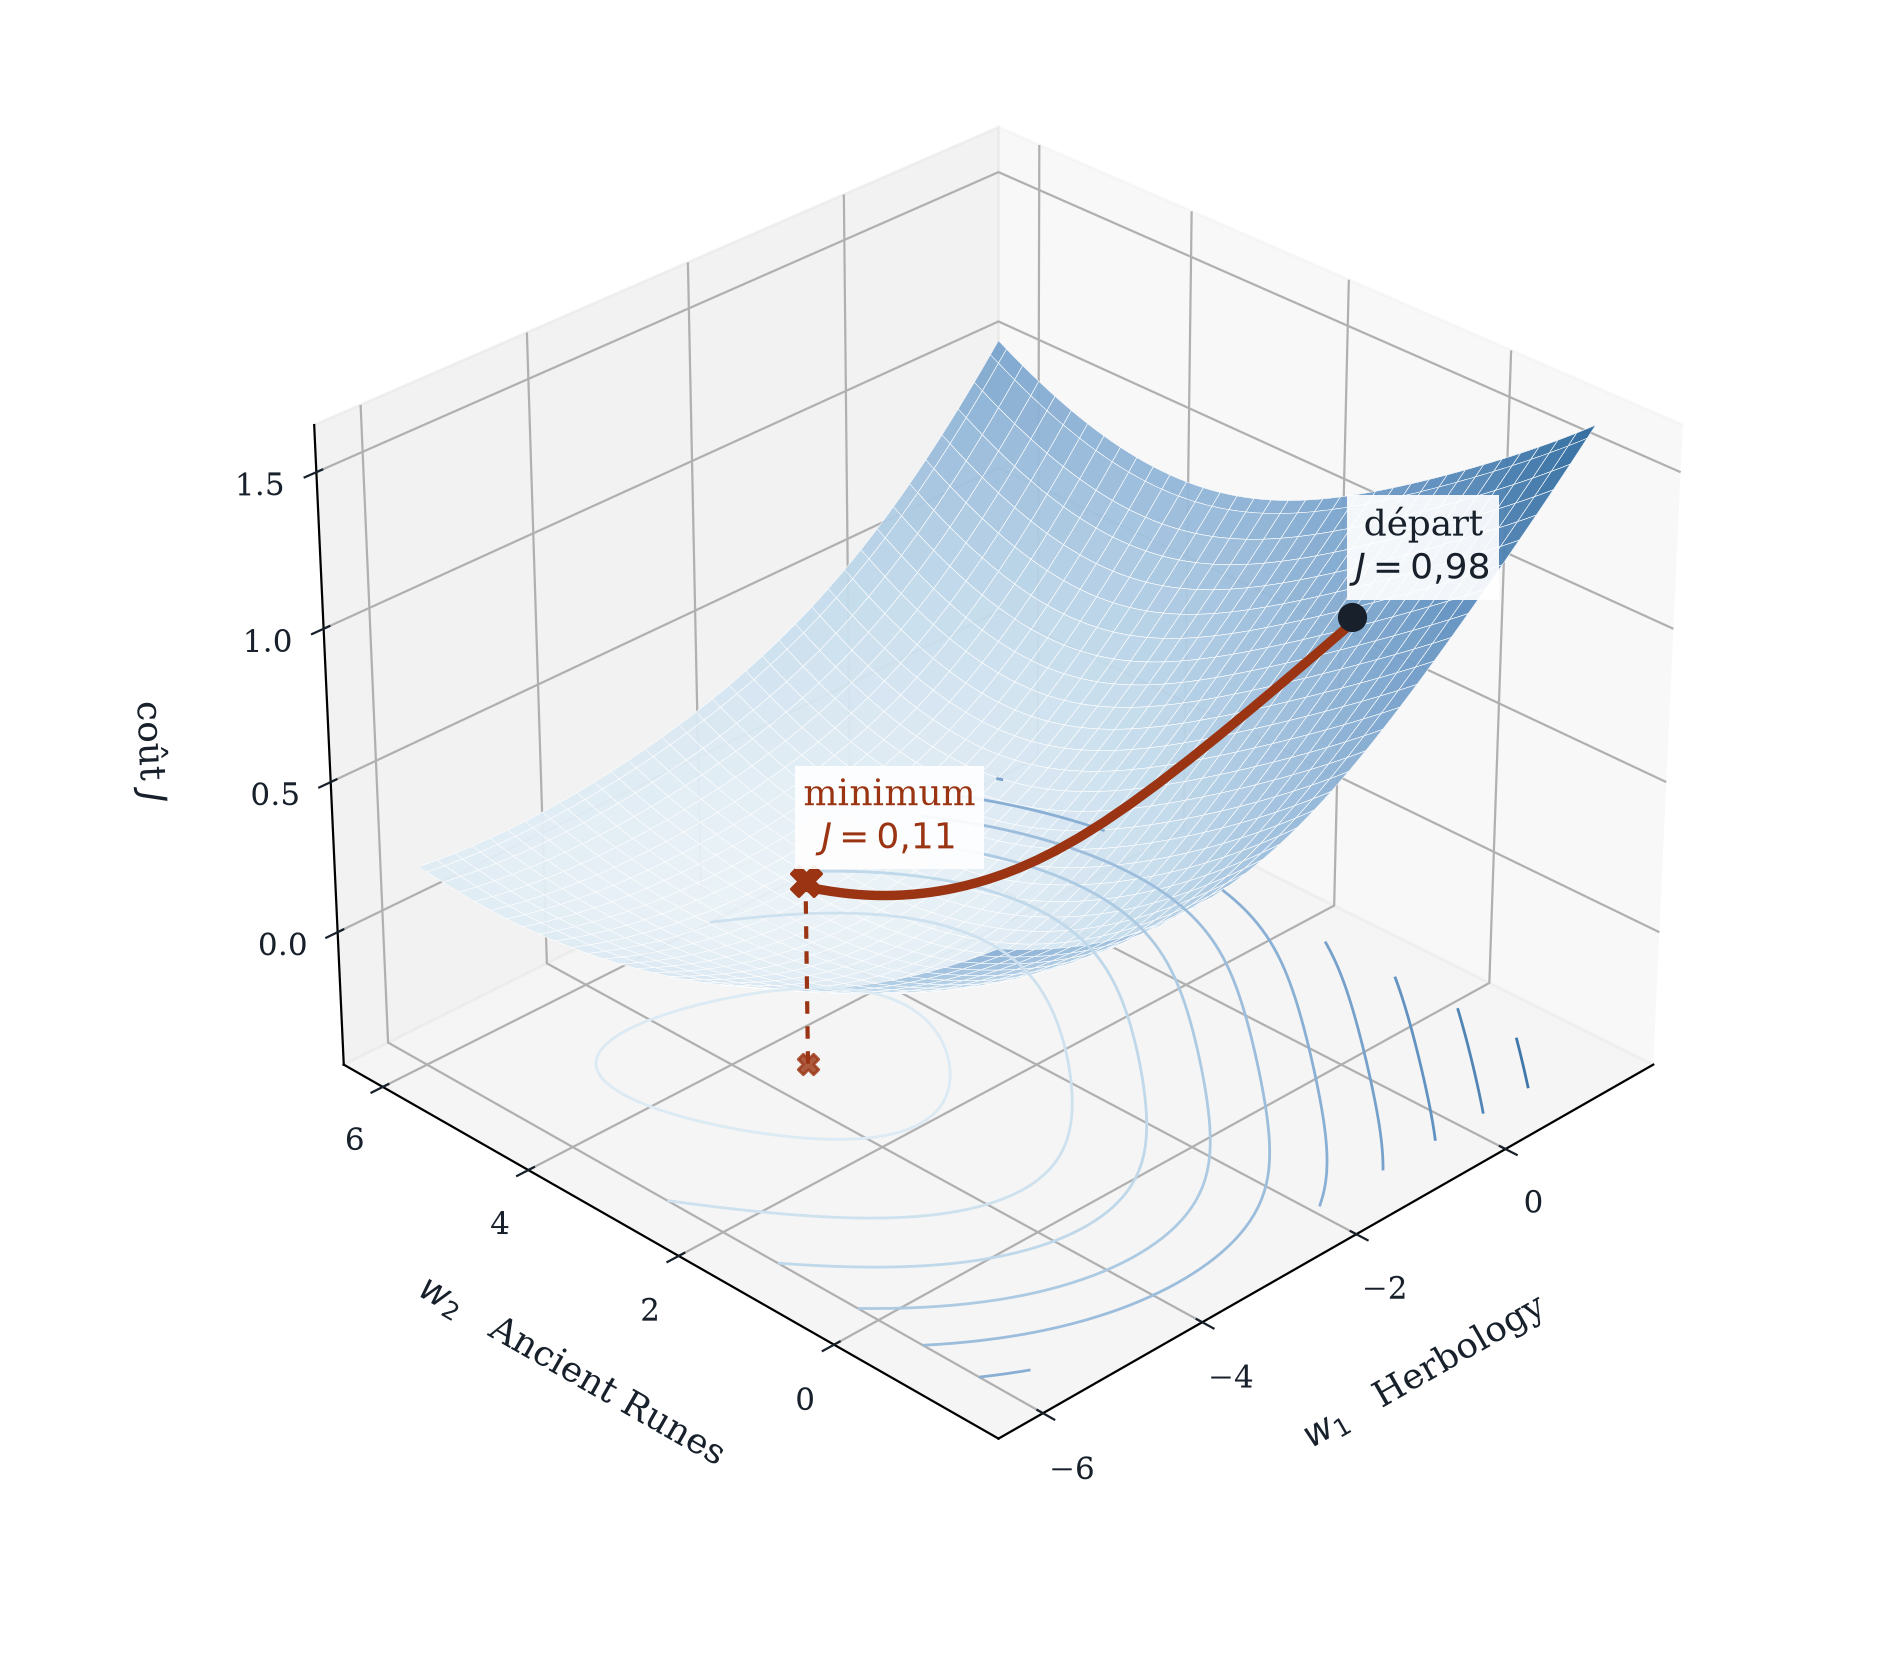
\includegraphics[width=1.12\textwidth]{figures/surface3d.png}}
\caption{La surface du coût au-dessus du plan $(w_1,w_2)$, le biais étant figé à
sa valeur finale. Chaque point du plan horizontal est un couple de coefficients,
et l'altitude au-dessus de lui est le coût que ce couple produit sur les $1\,600$
élèves. La trajectoire rouge part des coefficients nuls et rejoint le
fond. Les courbes tracées au sol sont les lignes de niveau, reprises seules à la
figure~\ref{fig:contours}, où la trajectoire se lit sans perspective.}
\label{fig:surface}
\vspace*{\fill}
\end{figure}

\begin{figure}[htbp]
\centering
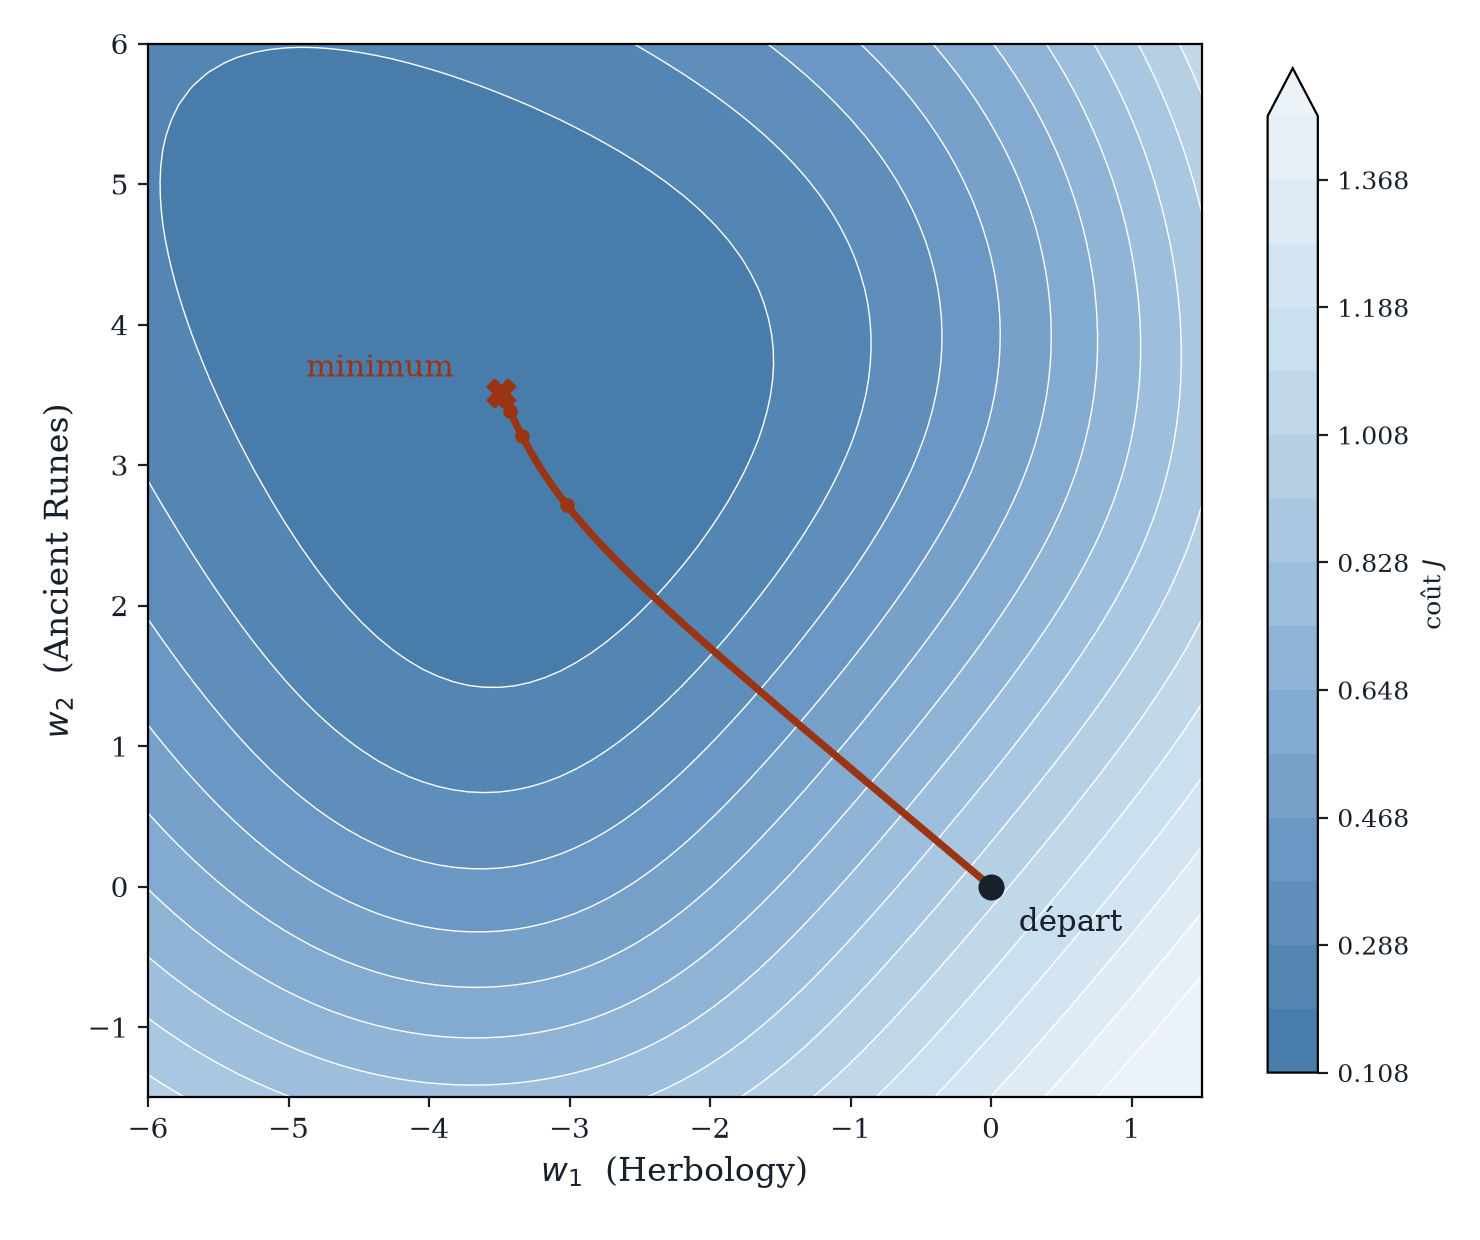
\includegraphics[width=.78\textwidth]{figures/contours.png}
\caption{La même surface vue de dessus. Chaque courbe relie les points de coût
égal, et la trajectoire les coupe perpendiculairement : c'est la propriété du
gradient, qui pointe dans la direction de plus forte pente. Les points marquent
une itération sur vingt-cinq, ce qui rend visible le ralentissement : les
premiers pas traversent plusieurs niveaux, les derniers se resserrent au fond.}
\label{fig:contours}
\end{figure}
\FloatBarrier

\begin{releve}
Le coût passe de $0{,}98$ aux coefficients nuls à $0{,}11$ au minimum, le biais
étant figé à sa valeur finale.
\end{releve}

\section{Longueur du pas}

À chaque tour, le gradient fournit une direction : celle dans laquelle le coût
décroît le plus vite depuis le point où l'on se trouve. Il reste muet sur la
distance à parcourir dans cette direction, et c'est $\alpha$ qui la fixe, en
multipliant le déplacement. Direction et longueur sont deux décisions séparées :
la première se calcule, la seconde se règle.

Un pas court avance peu à chaque tour. La correction disponible n'est consommée
que par fractions, et il en faut d'autant plus pour parcourir la même distance.
Comme un tour demande un passage complet sur les $1\,600$ élèves, le prix se paie
en temps de calcul, pour aboutir à la même frontière.

Un pas long expose au dépassement. Or la pente que donne le gradient ne décrit
fidèlement le terrain qu'au voisinage du point où elle est calculée. Sortir de ce
voisinage fait passer les coefficients de l'autre côté du minimum, sur la pente
opposée, si bien que le coût augmente au lieu de baisser
(figure~\ref{fig:alpha}). Les tours suivants ramènent vers le bas, mais la
trajectoire a fait un détour.

\begin{figure}[htbp]
\centering
\begin{tikzpicture}
\begin{axis}[width=.82\textwidth,height=6.8cm,
  axis lines=left,axis line style={ink!40},
  grid=major,grid style={gridgray!30},
  tick label style={font=\small},label style={font=\small},
  xlabel={itération},ylabel={coût $J$},
  xmin=0,xmax=40,ymin=0.09,ymax=0.72,
  legend style={at={(0.98,0.97)},anchor=north east,draw=none,font=\small,
    fill=white,fill opacity=0.85,text opacity=1}]
  \addplot[warning,very thick,no markers] table[x=iter,y=a005] {data/alpha.dat};
  \addlegendentry{$\alpha=0{,}05$}
  \addplot[huffle,thick,densely dashed,no markers]
    table[x=iter,y=a03] {data/alpha.dat};
  \addlegendentry{$\alpha=0{,}3$}
  \addplot[accent,very thick,no markers] table[x=iter,y=a10] {data/alpha.dat};
  \addlegendentry{$\alpha=1$}
  \addplot[slyth,thick,densely dotted,no markers]
    table[x=iter,y=a1000] {data/alpha.dat};
  \addlegendentry{$\alpha=100$}
\end{axis}
\end{tikzpicture}
\caption{Quarante itérations sur les $1\,600$ élèves, à partir des mêmes
coefficients nuls. Le pas le plus court laisse la courbe très au-dessus des
autres : il lui faudrait des centaines de tours pour les rejoindre. Le pas le
plus long fait remonter le coût dès le premier déplacement, avant de redescendre.}
\label{fig:alpha-reel}
\end{figure}
\FloatBarrier

\begin{chiffres}[Coût moyen selon le pas]
\begin{center}
\begin{tabular}{crrrl}
\toprule
$\alpha$ & départ & après un tour & après quarante & \\
\midrule
$0{,}05$ & $0{,}693$ & $0{,}684$ & $0{,}467$ & pas trop court \\
$0{,}3$  & $0{,}693$ & $0{,}642$ & $0{,}238$ & \\
$1$      & $0{,}693$ & $0{,}539$ & $0{,}153$ & réglage retenu \\
$100$    & $0{,}693$ & $0{,}408$ & $0{,}112$ & dépassement au premier pas \\
\bottomrule
\end{tabular}
\end{center}
Les quatre partent du même coût, $\log 2=0{,}693$, puisque les coefficients
nuls donnent $0{,}5$ à tout le monde. À $\alpha=0{,}05$, atteindre $0{,}15$
demanderait plusieurs centaines de tours pour la même frontière. À $\alpha=100$,
le premier pas emmène les coefficients au-delà du minimum, et la trajectoire
revient ensuite par l'autre versant : quarante tours plus tard, ce réglage a
rattrapé son détour et devancé $\alpha=1$. Ce rattrapage tient à une propriété
de ce coût précisément, établie ci-dessous.
\end{chiffres}

$\alpha$ se règle par essais, en lisant la courbe de coût : un bon réglage la
fait décroître à chaque tour, vite d'abord puis de moins en moins. On retient ici
$\alpha=1$.

\begin{vigilance}[Effet d'un pas excessif]
Le déplacement produit par un pas reste borné quel que soit $\alpha$ : la dérivée
du coût par rapport au score vaut $p-y$, de valeur absolue inférieure à $1$, et
la courbure est majorée par $p(1-p)\leq\frac14$. Un $\alpha$ excessif allonge la trajectoire au lieu de faire exploser les valeurs. Sur ces données,
$\alpha=1\,000$ porte le coût à $6{,}61$ au premier tour, puis le fait
redescendre tour après tour.
\end{vigilance}

\begin{figure}[htbp]
\centering
\begin{minipage}[t]{.48\textwidth}
\centering
\begin{tikzpicture}
\begin{axis}[width=.95\linewidth,height=5.4cm,axis lines=left,
  title={$\alpha$ adapté},xlabel={itération},ylabel={$\theta$},
  xmin=0,xmax=6,ymin=-2.6,ymax=6.6,grid=major,grid style={gridgray!45}]
  \addplot[accent,very thick,mark=*] coordinates
    {(0,-2) (1,0) (2,1) (3,1.5) (4,1.75) (5,1.875) (6,1.9375)};
  \addplot[ink,dashed,thick,domain=0:6]{2};
\end{axis}
\end{tikzpicture}
\end{minipage}\hfill
\begin{minipage}[t]{.48\textwidth}
\centering
\begin{tikzpicture}
\begin{axis}[width=.95\linewidth,height=5.4cm,axis lines=left,
  title={$\alpha$ trop grand},xlabel={itération},ylabel={$\theta$},
  xmin=0,xmax=6,ymin=-2.6,ymax=6.6,grid=major,grid style={gridgray!45}]
  \addplot[warning,very thick,mark=*] coordinates
    {(0,-2) (1,6) (2,-2) (3,6) (4,-2) (5,6) (6,-2)};
  \addplot[ink,dashed,thick,domain=0:6]{2};
\end{axis}
\end{tikzpicture}
\end{minipage}
\caption{Le cas général, sur une fonction quadratique d'une seule variable dont
le minimum est en $2$. À gauche le coefficient s'en approche, à droite il oscille
entre deux valeurs sans converger. Ce second comportement suppose une courbure
croissant avec la distance ; celle du coût logistique reste majorée par
$\frac14$.}
\label{fig:alpha}
\end{figure}
\FloatBarrier

\begin{resultat}[Critères d'arrêt]
Deux critères, employés ensemble. Le premier compare deux coûts successifs : si
la baisse relative passe sous $\varepsilon$, la descente a convergé. Le
second est un plafond d'itérations, qui borne le temps de calcul lorsque le
premier tarde à se déclencher. Sur les $1\,600$ élèves, la baisse relative passe
sous $10^{-6}$ bien après que la frontière a cessé de se déplacer
de façon perceptible : convergence numérique et stabilité des décisions sont deux
choses distinctes.
\end{resultat}
